\subsection{Continuity properties of the integral}

PROPOSITION 8. --- Suppose that E is Hausdorff; let \(\mu\) be a measure on X. The mapping \(\mathbf{f} \mapsto \int \mathbf{f} d\mu\) of \(\mathcal{K}(\mathrm{X};\mathbf{E})\) into \(\widehat{\mathbf{E}}\) (No.~3, Cor. 1 of Prop. 7) is the unique continuous linear mapping \(\Phi\) such that \(\Phi(g \cdot \mathbf{a}) = \mu(g) \cdot \mathbf{a}\) for every vector \(\mathbf{a} \in \mathbf{E}\) and every function \(g \in \mathcal{K}(\mathrm{X};\mathbf{C})\) .

To prove the continuity of the mapping \(f \mapsto \int f d\mu\) , it suffices to show that its restriction to \(\mathcal{K}(X, K; E)\) is continuous for every compact subset K of X (TVS, II, §4, No.~4, Prop. 5). We note that if the topology of E is defined by a family of semi-norms \((q_{\alpha})\) , that of \(\mathcal{K}(X, K; E)\) is defined by the family of semi-norms

\[
p _ {\alpha} (\mathbf {f}) = \sup _ {x \in K} q _ {\alpha} \bigl (\mathbf {f} (x) \bigr).
\]

Now, let h be a continuous mapping of X into \([0,1]\) , with compact support and such that \(h(x)=1\) on K; by No.~2, Prop. 6 we have, for every function \(\mathbf{f}\in\mathcal{K}(\mathrm{X},\mathrm{K};\mathrm{E})\) ,

\[
q _ {\alpha} \left(\int \mathbf {f} d \mu\right) = q _ {\alpha} \left(\int h \mathbf {f} d \mu\right) \leqslant \int h (x) q _ {\alpha} (\mathbf {f} (x)) d | \mu | (x) \leqslant | \mu | (h) \cdot p _ {\alpha} (\mathbf {f})
\]

(the \(q_{\alpha}\) being extended by continuity to \(\widehat{\mathbf{E}}\) ), which proves the continuity of \(\mathbf{f} \mapsto \int \mathbf{f} d\mu\) . On the other hand, with the notations of the statement,

\[
\int \left(g (x) \cdot {\bf a}\right) d \mu (x) = \mu (g) \cdot {\bf a}
\]

by virtue of No.~1, Example 1 and Prop. 2 of No.~2 applied to the canonical injection \(\mathbf{C} \cdot \mathbf{a} \to \mathrm{E}\) . Moreover, the subspace of \(\mathcal{K}(\mathrm{X};\mathrm{E})\) formed by the linear combinations \(\sum_{i} g_i \cdot \mathbf{a}_i\) , where \(\mathbf{a}_i \in \mathrm{E}\) and \(g_i \in \mathcal{K}(\mathrm{X};\mathbf{C})\) , is dense in \(\mathcal{K}(\mathrm{X};\mathrm{E})\) (§1, No.~2, Prop. 5), which completes the proof.

PROPOSITION 9. --- Suppose that E is Hausdorff; let f be a continuous mapping of X into E with compact support. When the space \(\mathcal{M}(\mathrm{X};\mathbf{C})\) is equipped with the topology of strictly compact convergence (§1, No.~10), the mapping \(\mu \mapsto \int \mathbf{f} d\mu\) of \(\mathcal{M}(\mathrm{X};\mathbf{C})\) into \(\widehat{\mathrm{E}}\) is the unique continuous linear mapping \(\Psi\) such that \(\Psi(\varepsilon_x) = \mathbf{f}(x)\) for all \(x \in \mathrm{X}\) .

For every \(\mathbf{z}' \in \mathrm{E}'\) ,

\[
\left\langle \int \mathbf {f} d \varepsilon_ {x}, \mathbf {z} ^ {\prime} \right\rangle = \int (\mathbf {z} ^ {\prime} \circ \mathbf {f}) d \varepsilon_ {x} = \mathbf {z} ^ {\prime} (\mathbf {f} (x)) = \langle \mathbf {f} (x), \mathbf {z} ^ {\prime} \rangle ,
\]

whence \(\int \mathbf{f} d\varepsilon_x = \mathbf{f}(x)\) . We know, moreover, that the set of point measures is total in \(\mathcal{M}(\mathrm{X};\mathbf{C})\) for the topology of strictly compact convergence (§2, No.~4, Cor. 4 of Th. 1). Thus it all comes down to proving the continuity of the linear mapping \(u: \mu \mapsto \int \mathbf{f} d\mu\) . For this, consider the linear mapping \(v: \mathbf{z}' \mapsto \langle \mathbf{f}, \mathbf{z}' \rangle\) of \(\mathrm{E}'\) into \(\mathcal{K}(\mathrm{X};\mathbf{C})\) , and let us show that the image under \(v\) of an equicontinuous subset H of \(\mathrm{E}'\) is contained in a strictly compact subset of \(\mathcal{K}(\mathrm{X};\mathbf{C})\) . For, if K is the support of \(\mathbf{f}\) , the functions \(\langle \mathbf{f}, \mathbf{z}' \rangle\) for \(\mathbf{z}' \in \mathrm{H}\) have support contained in K; on the other hand, these functions form an equicontinuous set, and for each \(x \in \mathrm{X}\) the set of \(\mathbf{z}'(\mathbf{f}(x))\) is bounded; our assertion therefore follows from Ascoli's theorem (GT, X, §2, No.~5, Cor. 3 of Th. 2). Now, it follows from formula (1) of No.~1 that \(u\) is none other than the restriction to \(\mathcal{M}(\mathrm{X};\mathbf{C})\) of the transpose \(^t v\) (in the algebraic sense); its continuity therefore follows from the foregoing (TVS, IV, §1, No.~3, Prop. 6).

COROLLARY. --- With hypotheses and notations as in Prop. 9, the restriction of the mapping \(\mu \mapsto \int \mathbf{f} d\mu\) to the set \(\mathcal{M}_{+}(\mathrm{X})\) of positive measures, or to a vaguely bounded subset B of \(\mathcal{M}(\mathrm{X};\mathbf{C})\) , is vaguely continuous.

For, it follows from §1, No.~10, Props. 17 and 18 that, on \(\mathcal{M}_{+}(X)\) or on B, the topology induced by the topology of strictly compact convergence is the same as the topology induced by the vague topology.

\pandocbounded{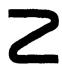
\includegraphics[keepaspectratio]{images/part001_df9b2198.jpg}}

However, the mapping \(\mu \mapsto \int \mathbf{f}d\mu\) is not necessarily continuous on all of \(\mathcal{M}(\mathrm{X};\mathbf{C})\) for the vague topology (Exer. 2).

